\section{Introduction}
\label{sec:intro}

Deep neural models have made remarkable strides in a broad spectrum 
of natural language understanding (NLU) 
tasks~\cite{bowman2015large,wang2018glue,mostafazadeh2016corpus,roemmele2011choice,zellers2018swag}. 
These tasks often employ a multiple-choice framework, as illustrated in \exref{exp:snli}. 
However, the inherent sensitivity of these models to minute variations 
calls for a robust and precise evaluation mechanism~\cite{checklist2020acl}.

\begin{center}
\begin{example}\label{exp:snli}
Natural language inference in the SNLI dataset, with the correct answer bolded.
\begin{description}
\item{Premise:} A swimmer playing in the surf watches a low flying airplane headed inland.
\item{Hypothesis:} Someone is swimming in the sea.
\item{Label:} \textbf{a) Entailment.} b) Contradiction. c) Neutral.
\end{description}
\end{example}
\end{center}

In tasks akin to \exref{exp:snli}, humans typically rely on the 
logical relationship between the premise and hypothesis. 
Contrarily, some NLP models might bypass this logical reasoning, 
focusing instead on the biases embedded within the dataset and, 
more specifically, within the hypotheses~\cite{naik2018stress,schuster2019towards}. 
These biases—such as sentiment or shallow n-grams—could provide misleading cues for correct predictions.

We refer to these biases as ``artificial spurious cues'' 
when they pervade both the training and test datasets, 
maintaining a similar distribution over predictions. 
An example of such a cue is a model's disproportionate 
dependence on the word ``someone'' in~\exref{exp:snli}. 
These cues, when absent or altered, can significantly impair a model's performance, 
underlining the importance of identifying them to enhance model robustness in the future.

\begin{figure}[th]
\centering
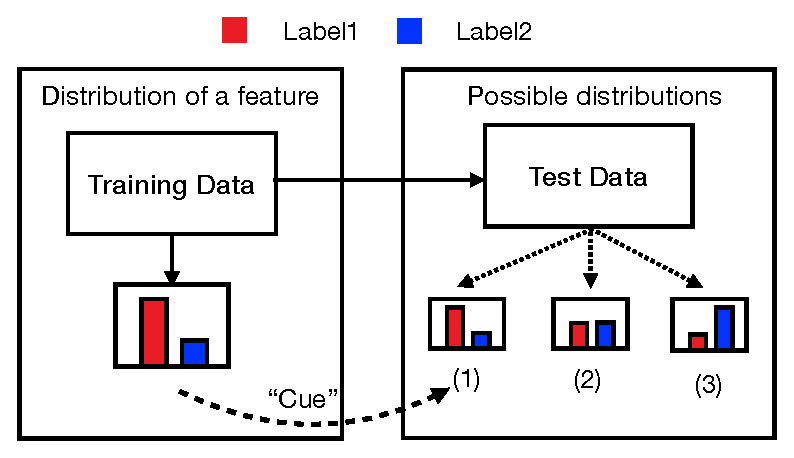
\includegraphics[width=0.70\columnwidth]{picture/cue_def.eps}
\caption{Example of a {\em cue}. }
\label{fig:cue_def}
\end{figure}

To tackle the issue of cues, it's crucial to distinguish between cues embedded 
in the dataset and those learned by the model. 
Conventional bias detection and mitigation tools, 
such as the AI Fairness 360 toolkit~\cite{bellamy2018ai}, 
primarily target dataset biases, 
inadequately addressing those learned by models during training.

While existing methods like ``hypothesis-only'' tests and 
CheckList can uncover model vulnerabilities, 
they're not expressly designed to identify model-learned cues. 
``Hypothesis-only'' tests can highlight dataset issues where 
the hypothesis alone can provide a correct answer 
but fail to realistically depict the model's capabilities as they 
don't evaluate the model using the full data context 
used during both training and prediction.

Drawing from the tenets of black-box testing in software engineering, 
CheckList scrutinizes model weaknesses without detailed knowledge of 
the model's internal architecture. It achieves this by delivering 
additional stress test cases premised on predefined linguistic features. 
However, CheckList's dependence on meticulously designed templates 
limits its scope, and it also falls short of 
illuminating the knowledge the model has actually gleaned from the data.

To address these limitations, we introduce ICQ (``I-see-cue''), 
a resilient statistical analysis framework~\footnote{The code and dataset are
available at \url{https://github.com/flora336/icq}}
%\KZ{Please include the real github url here: \url{http://anonymized.for.blind.review}}}
engineered to identify model-learned cues. 
Diverging from traditional methods, 
ICQ identifies biases in multiple-choice NLU datasets without necessitating additional 
test cases. Employing black-box testing, ICQ assesses how models utilize 
these biases, delivering a comprehensive understanding of the bias in NLU tasks.

We authenticate ICQ's efficacy by deploying it on various 
NLU datasets to probe potential cues learned by models during training. 
ICQ facilitates an in-depth understanding of how models like ChatGPT~\footnote{\url{https://chat.openai.com/}} 
learn potential cues, and it offers illustrative examples to guide the selection of suitable prompts, providing invaluable guidance for model optimization.

In summary, this paper contributes the following:

\begin{itemize}
\item We unveil ICQ, a lightweight yet potent method for identifying statistical biases and cues in NLU datasets, proposing simple and efficient tests to quantitatively and visually evaluate whether a model leverages spurious cues in its predictions.
\item We execute a comprehensive evaluation of statistical bias issues across ten popular NLU datasets and four models, corroborating previous findings and unveiling new insights. We also offer an online demonstration system to showcase the results and invite users to evaluate their own datasets and models.
\item Through a case study, we delve into how ChatGPT learns potential biases, offering valuable recommendations for its practical applications.
\end{itemize}





%Deep neural models have demonstrated efficacy in various natural 
%language understanding (NLU) tasks~\cite{bowman2015large,wang2018glue,mostafazadeh2016corpus,roemmele2011choice,zellers2018swag}. 
%Many tasks involve categorizing outcomes in multiple-choice settings, 
%as exemplified in \exref{exp:snli}. Accurate evaluation of these models is paramount, 
%given their susceptibility to minor perturbations~\cite{checklist2020acl}.
%
%\begin{center}
%\begin{example}\label{exp:snli}
%Natural language inference in SNLI dataset, with ground truth bolded.
%\begin{description}
%\item{Premise:} A swimmer playing in the surf watches a low flying airplane headed inland. 
%\item{Hypothesis:} Someone is swimming in the sea.
%\item{Label:} \textbf{a) Entailment.} b) Contradiction.  c) Neutral.
%\end{description}
%\end{example}
%\end{center}
%
%In \exref{exp:snli}, the logical connection between the premise and 
%the hypothesis is what humans rely on to solve the problem. 
%However, some NLP models~\cite{naik2018stress,schuster2019towards} 
%may sidestep this reasoning process and solve the problem by 
%focusing solely on dataset hypotheses. 
%The reason for this is the presence of inherent biases 
%in artificially constructed hypotheses, which are predictive of correct answers. 
%These biases often originate from the dataset, 
%and manifest as statistical correlations, such as sentiment, or shallow n-grams. 
%
%In the context of this paper, we term these biases ``artificial spurious cues'' 
%when they appear both in the training and test datasets 
%with a similar distribution over the prediction values, 
%as illustrated in~\figref{fig:cue_def}. 
%For example, the over-reliance on the word ``no'' by a model 
%could be an artifact of such cues present in the dataset. 
%If a model overly depends on these cues for predictions, 
%its performance could deteriorate when these cues are absent or altered. 
%This lack of robustness underscores the need for model 
%training and evaluation approaches that can effectively identify and 
%mitigate the influence of such biases, 
%thereby improving the overall reliability and fairness of AI systems.
%
%
%
%\begin{figure}[th]
%\centering
%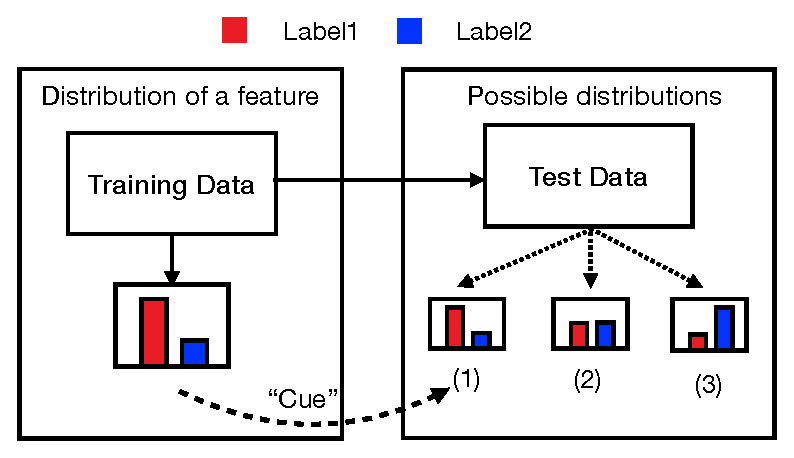
\includegraphics[width=0.70\columnwidth]{picture/cue_def.eps}
%\caption{Example of a {\em cue}. }
%\label{fig:cue_def}
%\end{figure}
%
%This brings us to an important distinction between different types of cues - dataset cues versus model-learned cues. In the context of AI fairness, tools such as the AI Fairness 360 toolkit~\cite{aif360-oct-2018} predominantly focus on dataset bias. However, our work with the ICQ (``I-see-cue'') framework aims to tackle model-learned biases that are induced from the data. By highlighting this distinction, we provide a more nuanced understanding of bias in NLU tasks, contributing to the ongoing discussion in the field.
%
%
%As we mentioned above, ``hypothesis-only'' tests can identify dataset issues 
%when questions can be answered correctly without the premise.
%However, they cannot validate the model's ability to answer questions without a 
%premise due to 
%a) it doesn't explain the cause of the model's problems, 
%and b) it doesn't directly evaluate the model, 
%as models use complete data during training and prediction, 
%making ``hypothesis-only'' tests unrealistic.
%
%Inspired by black-box testing in software engineering, 
%CheckList~\cite{checklist2020acl} 
%assesses model weaknesses without requiring detailed knowledge 
%of the model by providing additional stress test cases based 
%on predefined linguistic features. 
%However, CheckList has limitations due to 
%the need for carefully crafted templates with 
%substantial restrictions, which limits the 
%testing space and complicates implementation. 
%Moreover, while CheckList identifies what the model cannot do, 
%it fails to shed light on what the model has actually learned from the data.
%
%To make full use of existing test sets and overcome the limitations of existing approaches, we propose ICQ, a lightweight, general statistical analysis framework. ICQ can identify biases in multiple-choice NLU datasets without requiring additional test cases, and evaluates how models exploit these biases using black-box testing.
%To address the above limitations of existing approaches and 
%fully utilize existing test sets, we propose ICQ (``I-see-cue''), 
%a lightweight, general statistical analysis framework. 
%ICQ identifies biases in multiple-choice NLU datasets 
%without the need for additional test cases and evaluates 
%how models exploit these biases through black-box testing. 
%As an open-source evaluation framework~\footnote{\url{http://anonymized.for.blind.review}}, 
%ICQ allows for the assessment of both datasets and their 
%corresponding models by extracting multiple test sets 
%from different perspectives within a single dataset.
%
%We validate ICQ's effectiveness on various NLU datasets 
%to investigate whether models have learned potential bias 
%information during training. 
%By employing the ICQ framework, 
%we gain a better understanding of ChatGPT~\footnote{\url{https://chat.openai.com/}}'s 
%learning of potential biases and discuss, 
%through examples, how to select appropriate prompts, 
%ultimately providing 
%valuable guidance for model optimization.
%
%
%In summary, this paper makes the following contributions:
%\begin{itemize}
%\item we present a lightweight yet effective method to uncover statistical biases and cues in NLU datasets, and propose two simple tests for quantitatively and visually evaluating whether a given model exploits spurious cues in its predictions.
%
%\item we conduct a comprehensive evaluation of statistical bias issues on 10 popular NLU datasets and 4 models, confirming previous findings and uncovering new insights, while also providing an online demonstration system to showcase the results and encourage users to assess their own datasets and models.
%\item we investigate ChatGPT's bias through a case 
%study and offer valuable recommendations for practical applications.
%
%\end{itemize}
%% (\secref{sec:result}).
%
%%\item We filter the training data and get a better performance on the \textbf{hard} dataset.
%%to get a high quality training dataset which
% %is possibly closer to the intended task. 
%
%
%
%
%
%
%
